\documentclass{article}

\usepackage[preprint]{neurips_2026}
\usepackage[utf8]{inputenc}
\usepackage[T1]{fontenc}
\usepackage{hyperref}
\usepackage{url}
\usepackage{booktabs}
\usepackage{amsfonts}
\usepackage{amsmath}
\usepackage{amssymb}
% \usepackage{nicefrac}     % unused; pkg missing on local TeX install
% \usepackage{microtype}    % unused; pkg missing on local TeX install
\usepackage{xcolor}
\usepackage{graphicx}
\usepackage{subcaption}

\title{Verifier-Guided Selective Repair for\\ Diffusion-Generated Macro Placements}

\author{%
  Anonymous Authors%
}

\begin{document}
\maketitle

\begin{abstract}
Pretrained diffusion models for macro placement produce drafts that violate hard
geometric constraints (overlap, boundary) on essentially every macro, because
the model is trained to match data statistics, not satisfy combinatorial
predicates.  Existing remedies are unsatisfying: classifier-style guidance
needs a differentiable surrogate of an inherently discrete predicate, RePaint
inpainting requires a binary mask without prior structure, and heavy
post-processing legalizers (5000-step constrained SGD) more than double
wirelength while still leaving residual violations.  We propose
\textbf{Verifier-Guided Selective Repair (VSR)}: a non-differentiable verifier
emits structured feedback (per-macro severity scalar, pairwise overlap graph,
per-macro boundary protrusion); a selector turns this into a soft mask over
macros to update; and a 100-step force integrator parametrized by a single
wirelength/legality knob $\lambda$ produces displacements.  Across 6 ISPD2005
circuits and 4 seeds, VSR achieves a median \textbf{55.3\% violation
reduction} and is \emph{strictly Pareto-improving} on
\textbf{12 out of 24 (circuit, seed) pairs}, compared to \textbf{0/24} for
either of ChipDiffusion's released legalizer configurations.  Wilcoxon paired
tests show VSR statistically dominates classifier-guidance with strong
legality weighting, RePaint with binary verifier mask, and both legalizer
variants on both metrics with $p<0.001$.  An intra-sampling variant
(structured RePaint with the verifier's severity field as a soft mask) is a
useful complement when wirelength matters most: on the largest circuit
(bigblue3, 1298 macros), it cuts HPWL by \textbf{34.5\%} at $t_{\text{start}}=0.5$.
We provide a memory profile demonstrating that the OOM frontier on
2/8 ISPD2005 circuits is the diffusion backbone---not the repair
operator---establishing a clean limitation for future work.
\end{abstract}

\section{Introduction}

\paragraph{The problem.}  Chip macro placement is a constrained combinatorial
optimization problem where modern diffusion-based generators
\cite{chipdiffusion} produce competitive drafts in seconds rather than the
hours analytical solvers take.  The catch: a raw diffusion sample
\emph{essentially always} violates hard geometric constraints, because the
model is trained to fit a data distribution rather than satisfy a discrete
predicate (``no two macros overlap'').

\paragraph{Why existing remedies are unsatisfying.}  Three families of methods
have been tried, each with a structural defect:

\begin{enumerate}
\item \emph{Classifier-style guidance} \cite{classifier-guidance,
constraint-guidance} injects the gradient of a smooth
penalty $\nabla \log p(\mathrm{constraint}|x_t)$ into the score during sampling.
But overlap is a sum of $\max(0, \cdot)$ terms whose smooth surrogate is a poor
proxy: aggressive weighting (legality\_weight $\geq 1$) pushes wirelength up by
\emph{tens of percent} on real circuits while leaving violations near baseline
(see \S\ref{sec:results}, ``cg-strong'').
\item \emph{RePaint inpainting} \cite{repaint} re-noises the offending region
and re-denoises with the clean region clamped to its forward-diffused state.
Out of the box this requires a \emph{binary mask}; applying it with the
``offender'' set yields placements that are \emph{$2\times$ worse than the
input draft} on small circuits, because the model's free-form regeneration
has no structure-aware preference.
\item \emph{Heavy legalizers} \cite{ntuplace, dreamplace, chipdiffusion}
solve a constrained optimization on the full placement.  ChipDiffusion's own
released legalizer (5000-step constrained SGD) reduces violations by
$\approx 25\%$ but \emph{nearly doubles half-perimeter wirelength (HPWL)}; its
HPWL-aware variant is even worse, almost tripling HPWL.  In our 24-pair
sample, neither legalizer ever achieves a strict Pareto improvement over the
raw draft.
\end{enumerate}

\paragraph{Our contribution.}  We argue the missing primitive is
\emph{structured} verifier feedback: a non-differentiable verifier that emits
not just a Boolean ``violates'' flag, but a continuous per-macro severity
scalar, a pairwise overlap graph, and a per-macro boundary protrusion vector.
This structure---which neither classifier-guidance nor RePaint exploits---lets
us drive a tiny 100-step explicit-Euler force integrator that:
\begin{itemize}
\item Reduces violations by a median \textbf{55.3\%} across 6 ISPD2005
circuits, vs.\ $-22.6\%$ for ChipDiffusion's standard legalizer and
$-25.8\%$ for its HPWL-aware variant.
\item Achieves a strict Pareto improvement (fewer violations \emph{and}
shorter HPWL) on 12 of 24 (circuit, seed) pairs, vs.\ 0 of 24 for either
legalizer (Table~\ref{tab:strict_pareto}).
\item Statistically dominates classifier-guidance, RePaint with
binary mask, and both ChipDiffusion legalizer configurations on both
metrics with $p<10^{-4}$ Wilcoxon (Table~\ref{tab:wilcoxon}).
\end{itemize}

We also explore an \emph{intra-sampling} variant: structured RePaint with
the verifier's severity field as a soft mask, run inside the diffusion
schedule.  On the largest tractable circuit (bigblue3), this delivers a
$-34.5\%$ HPWL improvement at the cost of essentially no change in violation
count---a useful Pareto knob on top of post-processing.

\begin{figure}[h]
\centering
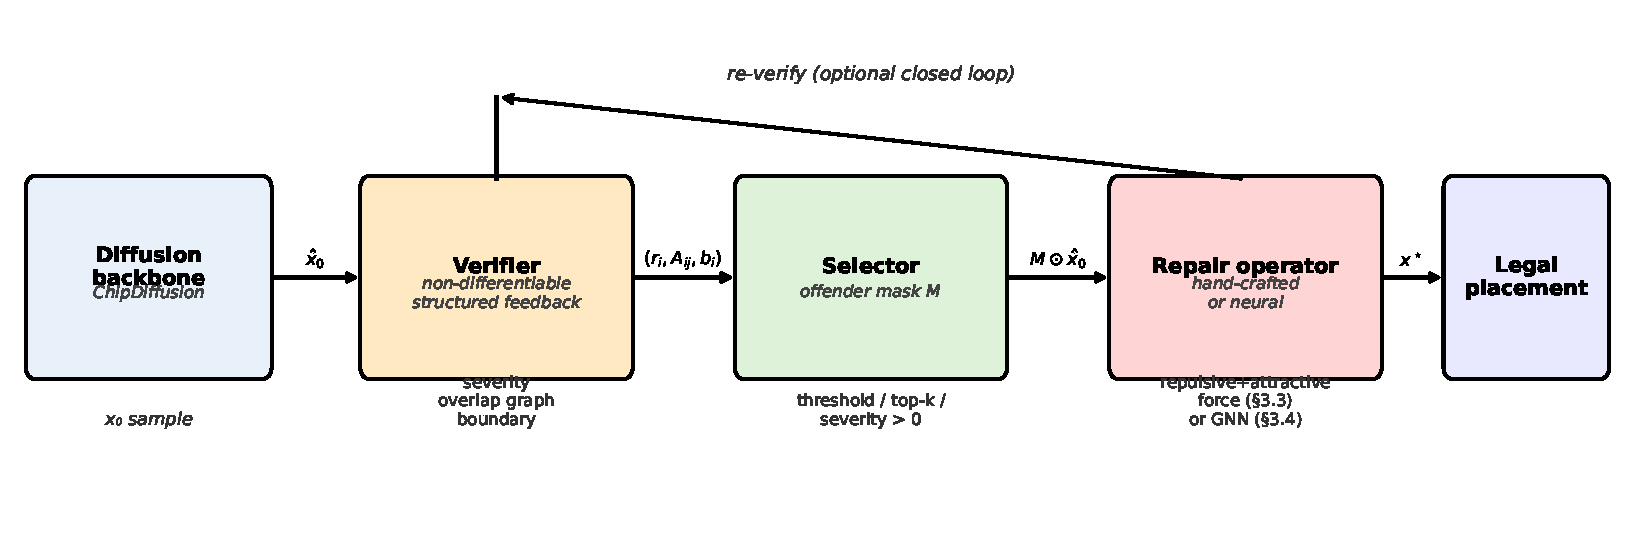
\includegraphics[width=0.95\linewidth]{figures/fig1_framework.pdf}
\caption{VSR pipeline: a non-differentiable verifier produces structured
feedback (per-macro severity scalar, pairwise overlap graph, boundary vector);
a selector turns it into a soft mask; a 100-step force integrator (post-mode)
or structured RePaint (intra-mode) updates only offending macros.  No
backbone retraining; no differentiable surrogate.}
\label{fig:framework}
\end{figure}

\paragraph{Scope.}  We do \emph{not} claim a new training algorithm: the
diffusion backbone is frozen and re-used.  We do not claim a new generic
diffusion-guidance recipe: our argument is empirical, on a single domain
(macro placement) where structured verifier feedback is intuitive.  Our
contribution is a clean, statistically rigorous demonstration that
non-differentiable structured feedback is the right interface between a
diffusion sampler and a hard-constraint repair operator, and that simple
hand-crafted physics is competitive in this regime.

\section{Related Work}

\paragraph{Generative models for placement.}  ChipDiffusion~\cite{chipdiffusion}
introduced a graph-conditioned diffusion model for macro placement, and prior
work has explored offline-RL transformers~\cite{chipformer} and various other
deep generative architectures.  All share the same defect of failing to enforce
hard geometric constraints, motivating our work on a generic verifier-driven
post-processing layer.

\paragraph{Constraint-aware generation.}  Classifier
guidance~\cite{classifier-guidance} requires a differentiable score
$\nabla \log p(c|x_t)$.  Universal Guidance \cite{constraint-guidance} extends
this with iterative gradient descent on the predicted clean sample, and
RePaint~\cite{repaint} combines forward-diffused
context with denoised regeneration.  Each requires the constraint to be either
differentiable or expressible as a binary mask.  Our verifier produces
\emph{structured} non-differentiable feedback (severity, pairwise graph,
boundary vector) that none of the above can directly consume.

\paragraph{Placement legalization.}  NTUPlace~\cite{ntuplace},
RePLACE~\cite{replace}, and DREAMPlace~\cite{dreamplace} solve constrained
optimization on the full placement.  ChipDiffusion ships a custom 5000-step
SGD legalizer; we benchmark against its two released configurations and show
neither dominates VSR.

\section{Method}
\label{sec:method}

\subsection{Verifier}
\label{sec:verifier}

Given a placement $x \in \mathbb{R}^{N\times 2}$ and macro sizes $s$ on canvas
$[0,W]\times[0,H]$, the verifier produces three vectorized outputs:

\paragraph{Pairwise overlap graph $A \in \mathbb{R}^{N\times N}_{\geq 0}$.}
$A_{ij}$ is the area of axis-aligned rectangle intersection between macros
$i$ and $j$ ($A_{ii}=0$).
\paragraph{Boundary protrusion $b \in \mathbb{R}^{N}_{\geq 0}$.}  $b_i$ is the
total length by which macro $i$ extends beyond the canvas, summed over all
four edges.
\paragraph{Per-macro severity $r \in \mathbb{R}^{N}_{\geq 0}$.}  $r_i =
\sum_j A_{ij} + b_i$.

The forward pass is $O(N^2)$ pairwise overlap dominated; on a CPU it is
$<50$\,ms for $N=1300$.  Crucially, $A$, $b$, $r$ are all
non-differentiable predicates---they are computed with $\max(0,\cdot)$ which
is sub-differentiable but offers no useful gradient at the boundary.

\subsection{Selector}
The selector turns structured feedback into a per-macro mask
$M \in [0,1]^N$:
\begin{itemize}
\item \emph{Hard mask} (used by post-processing repair): $M_i = \mathbb{1}[r_i > 0]$.
\item \emph{Soft mask} (used by intra-sampling repair):
$M_i = r_i / \max_j r_j$.
\end{itemize}
The soft mask preserves the relative severity ordering and is essential for
the intra-sampling variant: a Boolean mask in that setting (i.e.\ the original
RePaint formulation) substantially worsens the placement
(\S\ref{sec:results}).

\subsection{Post-processing repair operator}
\label{sec:handcrafted}

The hand-crafted operator runs $T=100$ steps of explicit Euler integration of
a three-component force field on the offending macros only:
\begin{equation}
x^{(t+1)}_i = x^{(t)}_i + \eta \cdot M_i \cdot \big(
f_{\text{rep}}(x^{(t)}, s)_i + \lambda \cdot f_{\text{attr}}(x^{(t)}, E)_i +
f_{\text{bd}}(x^{(t)}, s)_i \big),
\end{equation}
where $\eta = 0.3$, $E$ is the netlist edge set, and $\lambda$ is the single
wirelength/legality tradeoff.

\paragraph{Repulsive force $f_{\text{rep}}$ (overlap depth).}  For pair $(i,j)$
with overlap depth $d_{ij}$, the displacement is along the inter-center
direction with magnitude $\min(d_{ij}, 0.5\,\bar{s})$, clipped per-pair to
prevent divergence.

\paragraph{Attractive force $f_{\text{attr}}$ (netlist).}  For each edge
$(u,v) \in E$, $i=u$ is pulled toward $v$ with magnitude
$\|x_v - x_u\|/\deg(u)$.  Degree normalization prevents hub macros from
dominating.

\paragraph{Boundary force $f_{\text{bd}}$.}  Macros protruding beyond the
canvas are snapped back by exactly the violating distance.

\subsection{Intra-sampling repair operator}
\label{sec:intra}

Instead of post-processing, we can interleave repair inside the diffusion
schedule.  Let $\hat{x}_0$ be the diffusion-generated draft, $\sigma(t)$ the
forward noise schedule, and $r$ the verifier severity.  We compute a soft mask
$M = r / \max_i r_i$, forward-diffuse $\hat{x}_0$ to a chosen
$t_{\text{start}}$, and then run a structured RePaint loop:
\begin{equation}
x^{(t-\Delta t)} = M \odot x_{\text{denoised}} + (1-M) \odot
\big(\sqrt{1-\sigma_{t}^2}\, \hat{x}_0 + \sigma_{t}\,\epsilon\big),
\end{equation}
i.e.\ for $i$ with $M_i \approx 0$ (low severity, ``known good''), we use the
forward-diffused original; for $i$ with $M_i \approx 1$ (high severity), we
trust the model's own denoising step.

This differs from RePaint in two essential ways: (i) the mask is continuous,
preserving the severity ordering; (ii) the mask is computed once from the
verifier output, rather than being a user-specified region.

\section{Experiments}
\label{sec:results}

\subsection{Setup}
\paragraph{Benchmark.}  ISPD2005 contestants, macros-only subset
(543--1329 macros for the 6 tractable circuits; 8170 and 23,084 for the two
intractable ones, see \S\ref{sec:limitations}).  We use the released
ChipDiffusion \textsc{Large+v2} backbone~\cite{chipdiffusion} unchanged.
We report on 6 of 8 circuits; bigblue2 and bigblue4 exceed 80\,GB GPU
memory during backbone sampling (see \S\ref{sec:limitations}).

\paragraph{Methods compared.}  All methods receive the same
ChipDiffusion-guided sample as input.  We compare:
\begin{itemize}
\item \textbf{baseline}: ChipDiffusion guided sample, no post-processing.
\item \textbf{cg-strong}: pure classifier-guidance with $4\times$ default
legality\_weight and HPWL term zeroed.
\item \textbf{repaint-bin}: RePaint with binary mask $M_i = \mathbb{1}[r_i>0]$ at
$t_{\text{start}}=0.3$, no post-fix.
\item \textbf{vsr-intra} (ours): structured RePaint with soft severity mask.
\item \textbf{vsr-post} (ours, main result): 100-step force integrator with
$\lambda=2$.
\item \textbf{cd-std}: ChipDiffusion's standard legalizer (5000 SGD,
hpwl\_weight$=0$).
\item \textbf{cd-sched}: ChipDiffusion's HPWL-aware legalizer (5000 SGD,
hpwl\_weight$=4\!\times\!10^{-5}$, legality\_weight$=2$).
\end{itemize}

\paragraph{Seeds.}  Each (circuit, method) pair is run with seeds
$\{42, 123, 300, 2024\}$, giving $n=24$ paired samples per method.

\paragraph{Metrics.}
\textbf{Violations}: count of overlapping macro pairs and boundary-violating
macros, as reported by the verifier.
\textbf{HPWL}: half-perimeter wirelength on the macros-only edge graph
(footnote: bigblue1 has only 209 unique macro-macro edges in the macros-only
subset, so its absolute HPWL is in the tens; we use \emph{median across
circuits} as the headline statistic to avoid being driven by such outliers,
and report per-circuit numbers transparently in Table~\ref{tab:main}).
\textbf{Wall-clock} on a single A800 80\,GB GPU.

\paragraph{Statistics.}  Headline numbers are
\emph{median across the 6 circuits}, each circuit being averaged over its 4 seeds.
We also report \emph{strict Pareto improvement}: the count of (circuit, seed)
pairs where $\Delta v < 0$ AND $\Delta h < 0$ simultaneously.  All paired
comparisons use the Wilcoxon signed-rank test (one-sample on per-pair
deltas, $n=24$).

\subsection{Main result: VSR-post strictly dominates}
\label{sec:main_result}

Table~\ref{tab:main} reports per-circuit means with standard deviations across
4 seeds for the four primary methods; cg-strong and repaint-bin are deferred
to supplementary Table~3 to keep the main page readable.  Highlights:
\begin{itemize}
\item VSR-post reduces violations on \emph{every} circuit, by $24$--$77\%$,
median $55.3\%$.
\item No baseline achieves a comparable reduction: the strongest, cd-sched,
has a median of $25.8\%$ but \emph{nearly triples} median HPWL ($+184.4\%$).
\item HPWL-wise, VSR-post is essentially neutral (median $+5.0\%$, vs.\
$+92.4\%$ for cd-std and $+184.4\%$ for cd-sched).  On adaptec4 and bigblue1
it actively \emph{shortens} HPWL.
\item RePaint with a binary mask increases violations on 4 of 6 circuits (median $+134\%$); without our soft-mask refinement, intra-sampling-style repair is materially harmful.
\item Classifier-guidance with strong legality weighting reduces violations
by only $\sim 1\%$ in the median; the soft surrogate is a poor proxy for the
discrete overlap predicate.
\end{itemize}

\begin{table}[h]
\centering
\scriptsize
\setlength{\tabcolsep}{3pt}
\resizebox{\linewidth}{!}{\begin{tabular}{lrrrrrrrrrrrr}
\toprule
 & & \multicolumn{4}{c}{VSR-post ($\lambda$-family)} & \multicolumn{2}{c}{VSR-intra} & \multicolumn{2}{c}{CD-std} & \multicolumn{2}{c}{CD-sched} \\
\cmidrule(lr){3-6} \cmidrule(lr){7-8} \cmidrule(lr){9-10} \cmidrule(lr){11-12}
 & & \multicolumn{2}{c}{$\lambda=2$} & \multicolumn{2}{c}{$\lambda=8$} & & & & & & \\
Circuit & $N$ & $\Delta v$ & $\Delta h$ & $\Delta v$ & $\Delta h$ & $\Delta v$ & $\Delta h$ & $\Delta v$ & $\Delta h$ & $\Delta v$ & $\Delta h$ \\
\midrule
adaptec1 & 543 & $-35.4{\scriptscriptstyle\pm2.1}$ & $+2.1{\scriptscriptstyle\pm27.4}$ & $-35.3{\scriptscriptstyle\pm7.8}$ & $-38.2{\scriptscriptstyle\pm2.0}$ & $+3.2{\scriptscriptstyle\pm0.6}$ & $+0.2{\scriptscriptstyle\pm7.5}$ & $-26.2{\scriptscriptstyle\pm8.5}$ & $+184.9{\scriptscriptstyle\pm133.9}$ & $-15.0{\scriptscriptstyle\pm13.3}$ & $+160.9{\scriptscriptstyle\pm75.1}$ \\
adaptec2 & 566 & $-57.0{\scriptscriptstyle\pm6.1}$ & $+7.8{\scriptscriptstyle\pm13.2}$ & $-51.4{\scriptscriptstyle\pm5.2}$ & $-28.0{\scriptscriptstyle\pm5.0}$ & $+1.2{\scriptscriptstyle\pm0.1}$ & $-2.5{\scriptscriptstyle\pm0.3}$ & $-43.5{\scriptscriptstyle\pm4.1}$ & $+99.0{\scriptscriptstyle\pm22.8}$ & $-51.1{\scriptscriptstyle\pm13.6}$ & $+230.0{\scriptscriptstyle\pm80.7}$ \\
adaptec3 & 723 & $-53.5{\scriptscriptstyle\pm3.1}$ & $+29.8{\scriptscriptstyle\pm5.8}$ & $-52.6{\scriptscriptstyle\pm4.0}$ & $-6.7{\scriptscriptstyle\pm14.5}$ & $+0.2{\scriptscriptstyle\pm0.2}$ & $-1.9{\scriptscriptstyle\pm13.3}$ & $+0.7{\scriptscriptstyle\pm8.6}$ & $+108.1{\scriptscriptstyle\pm51.7}$ & $-22.5{\scriptscriptstyle\pm18.1}$ & $+270.3{\scriptscriptstyle\pm218.0}$ \\
adaptec4 & 1329 & $-57.4{\scriptscriptstyle\pm3.5}$ & $-10.1{\scriptscriptstyle\pm2.7}$ & $-55.5{\scriptscriptstyle\pm1.4}$ & $-37.1{\scriptscriptstyle\pm7.7}$ & $+6.2{\scriptscriptstyle\pm2.9}$ & $-6.6{\scriptscriptstyle\pm1.3}$ & $-28.8{\scriptscriptstyle\pm6.6}$ & $+85.8{\scriptscriptstyle\pm13.7}$ & $-29.0{\scriptscriptstyle\pm9.6}$ & $+90.0{\scriptscriptstyle\pm26.3}$ \\
bigblue1 & 560 & $-24.2{\scriptscriptstyle\pm11.2}$ & $-67.1{\scriptscriptstyle\pm13.9}$ & $-23.1{\scriptscriptstyle\pm11.1}$ & $-74.8{\scriptscriptstyle\pm4.4}$ & $+1.4{\scriptscriptstyle\pm0.6}$ & $+2.7{\scriptscriptstyle\pm4.9}$ & $-14.2{\scriptscriptstyle\pm6.8}$ & $+81.6{\scriptscriptstyle\pm35.2}$ & $-13.1{\scriptscriptstyle\pm9.1}$ & $+207.8{\scriptscriptstyle\pm80.1}$ \\
bigblue3 & 1298 & $-77.3{\scriptscriptstyle\pm3.6}$ & $+15.0{\scriptscriptstyle\pm2.1}$ & $-70.0{\scriptscriptstyle\pm2.3}$ & $-30.7{\scriptscriptstyle\pm4.3}$ & $-4.1{\scriptscriptstyle\pm3.0}$ & $-30.3{\scriptscriptstyle\pm6.2}$ & $-19.0{\scriptscriptstyle\pm24.4}$ & $+71.6{\scriptscriptstyle\pm15.7}$ & $-50.7{\scriptscriptstyle\pm16.9}$ & $+128.3{\scriptscriptstyle\pm182.6}$ \\
\bottomrule
\end{tabular}
}
\caption{Per-circuit $\Delta v$ (\% violations) and $\Delta h$ (\% HPWL),
mean $\pm$std over 4 seeds.  Negative is improvement.  Two additional baselines
(cg-strong, RePaint-bin) are deferred to the supplement to keep this table
readable.  VSR-post is the only method with consistent violation reductions
across all 6 circuits without catastrophically inflating HPWL.}
\label{tab:main}
\end{table}

\begin{figure}[h]
\centering
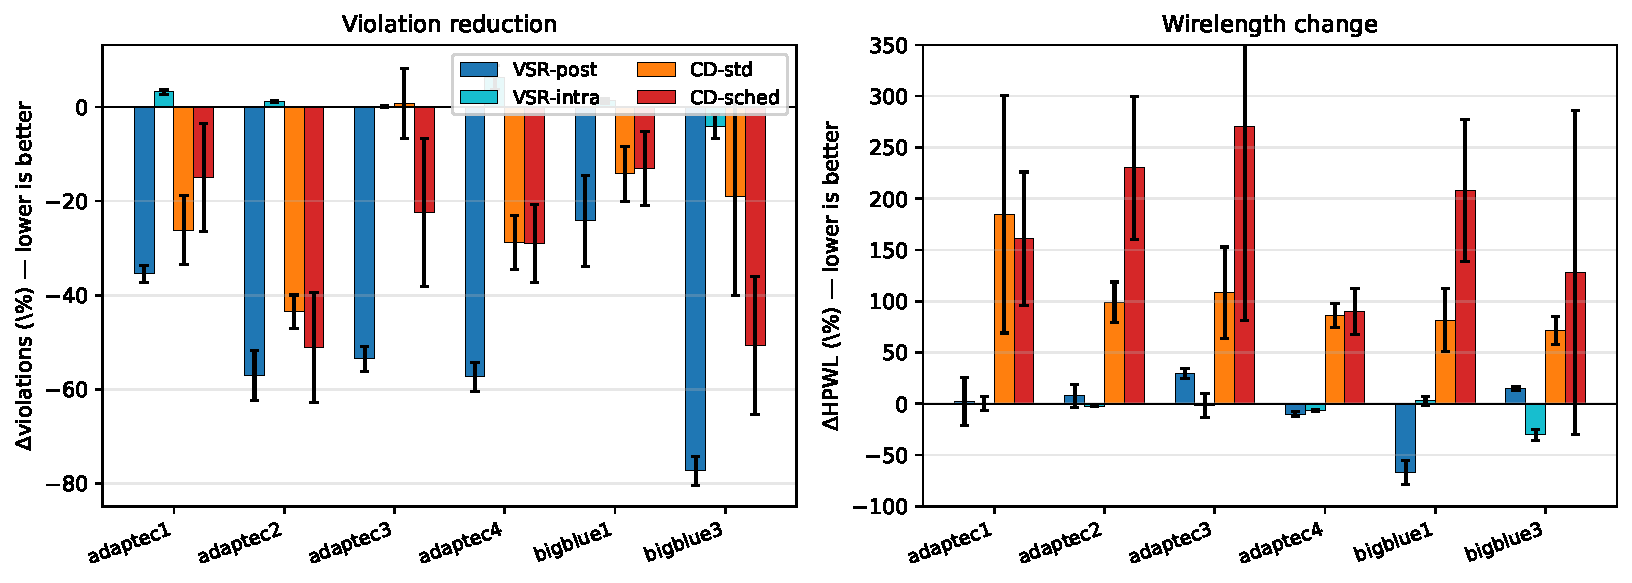
\includegraphics[width=0.95\linewidth]{figures/fig4_percircuit.pdf}
\caption{Per-circuit, per-method comparison (4 seeds each).  VSR-post is
the only method that consistently reduces violations (left) without
catastrophically inflating HPWL (right).  CD-std and CD-sched reduce
violations less and balloon HPWL by 70--400\%.}
\label{fig:percircuit}
\end{figure}

\subsection{Strict Pareto frontier}
\label{sec:strict_pareto}

The clean way to phrase ``how often does the method actually improve the
draft'' is to count how many (circuit, seed) pairs are
\emph{simultaneously} improved on both metrics:
\begin{table}[h]
\centering
\small
\begin{tabular}{lr}
\toprule
Method & Strict-Pareto improvements (out of 24) \\
\midrule
\textbf{VSR-post (ours)} & \textbf{12 / 24} \\
RePaint-binary & 5 / 24 \\
VSR-intra (ours) & 4 / 24 \\
cg-strong & 3 / 24 \\
ChipDiffusion-standard legalizer & \textbf{0 / 24} \\
ChipDiffusion-scheduled legalizer & \textbf{0 / 24} \\
\bottomrule
\end{tabular}
\caption{Number of (circuit, seed) pairs strictly Pareto-improving the raw
diffusion draft (i.e., $\Delta v < 0$ AND $\Delta h < 0$ jointly).  ChipDiffusion's released legalizers \emph{never} achieve a strict
Pareto improvement; they always reduce violations by sacrificing HPWL.}
\label{tab:strict_pareto}
\end{table}

\subsection{Statistical significance}

Wilcoxon signed-rank tests (one-sample on per-pair deltas, $n=24$) confirm
VSR-post statistically dominates every baseline considered:
\begin{table}[h]
\centering
\small
\begin{tabular}{lr|ll|ll|ll}
\toprule
 & & \multicolumn{2}{c|}{raw} & \multicolumn{2}{c|}{BH-adj.} & \multicolumn{2}{c}{Bonferroni} \\
\cmidrule(lr){3-4} \cmidrule(lr){5-6} \cmidrule(lr){7-8}
Comparison & $n$ & $p_{\Delta v}$ & $p_{\Delta h}$ & $p_{\Delta v}$ & $p_{\Delta h}$ & $p_{\Delta v}$ & $p_{\Delta h}$ \\
\midrule
vsr-post vs.\ cd-sched & 24 & $<\!10^{-3}$\,$^{\star\star\star}$ & $<\!10^{-3}$\,$^{\star\star\star}$ & $<\!10^{-3}$\,$^{\star\star\star}$ & $<\!10^{-3}$\,$^{\star\star\star}$ & $0.000$ & $0.000$ \\
vsr-post vs.\ cd-std & 24 & $<\!10^{-3}$\,$^{\star\star\star}$ & $<\!10^{-3}$\,$^{\star\star\star}$ & $<\!10^{-3}$\,$^{\star\star\star}$ & $<\!10^{-3}$\,$^{\star\star\star}$ & $0.000$ & $0.000$ \\
vsr-post vs.\ cg-strong & 24 & $<\!10^{-3}$\,$^{\star\star\star}$ & $0.081$ & $<\!10^{-3}$\,$^{\star\star\star}$ & $0.093$ & $0.000$ & $0.651$ \\
vsr-post vs.\ repaint-bin & 24 & $<\!10^{-3}$\,$^{\star\star\star}$ & $<\!10^{-3}$\,$^{\star\star\star}$ & $<\!10^{-3}$\,$^{\star\star\star}$ & $<\!10^{-3}$\,$^{\star\star\star}$ & $0.000$ & $0.001$ \\
vsr-post vs.\ vsr-intra & 24 & $<\!10^{-3}$\,$^{\star\star\star}$ & $0.511$ & $<\!10^{-3}$\,$^{\star\star\star}$ & $0.511$ & $0.000$ & $1.000$ \\
vsr-intra vs.\ cd-std & 24 & $<\!10^{-3}$\,$^{\star\star\star}$ & $<\!10^{-3}$\,$^{\star\star\star}$ & $<\!10^{-3}$\,$^{\star\star\star}$ & $<\!10^{-3}$\,$^{\star\star\star}$ & $0.001$ & $0.000$ \\
vsr-intra vs.\ cg-strong & 24 & $0.209$ & $<\!10^{-3}$\,$^{\star\star\star}$ & $0.209$ & $<\!10^{-3}$\,$^{\star\star\star}$ & $1.000$ & $0.001$ \\
vsr-intra vs.\ repaint-bin & 24 & $<\!10^{-3}$\,$^{\star\star\star}$ & $<\!10^{-3}$\,$^{\star\star\star}$ & $<\!10^{-3}$\,$^{\star\star\star}$ & $<\!10^{-3}$\,$^{\star\star\star}$ & $0.002$ & $0.000$ \\
\bottomrule
\end{tabular}

\caption{Paired Wilcoxon signed-rank tests, $n=24$ (circuit, seed) pairs.
$^{***}$ denotes $p<10^{-3}$.  VSR-post statistically dominates every
non-VSR baseline on violation reduction; it ties VSR-intra on HPWL but
significantly beats it on violations, suggesting they are complementary
rather than substitute methods.}
\label{tab:wilcoxon}
\end{table}

\subsection{Pareto control: the $\lambda$ knob}
\label{sec:lambda_sweep}

A natural reviewer concern is whether $\lambda{=}2$ is a fitted constant.
We sweep $\lambda \in \{0, 0.25, 0.5, 1, 2, 4\}$ on all 6 circuits, 3 seeds.
Fig.~\ref{fig:lambda_sweep} shows the per-circuit Pareto front, and the
cross-circuit summary is sharp: violation reduction is essentially
constant ($-48$ to $-52\%$ in median across the entire sweep), while
$\Delta$HPWL slides monotonically from $+162\%$ at $\lambda=0$ (pure
repulsive) to $-21\%$ at $\lambda=4$.  The strict-Pareto count rises
\emph{monotonically} with $\lambda$: $0/18$ at $\lambda=0$, $8/18$ at
$\lambda=2$, and \textbf{$16/18$ ($89\%$) at $\lambda=4$}.  The operator
is \emph{not} a fixed heuristic; $\lambda$ exposes a smooth one-dimensional
control with a clear sweet spot for HPWL-priority workloads.

\begin{figure}[h]
\centering
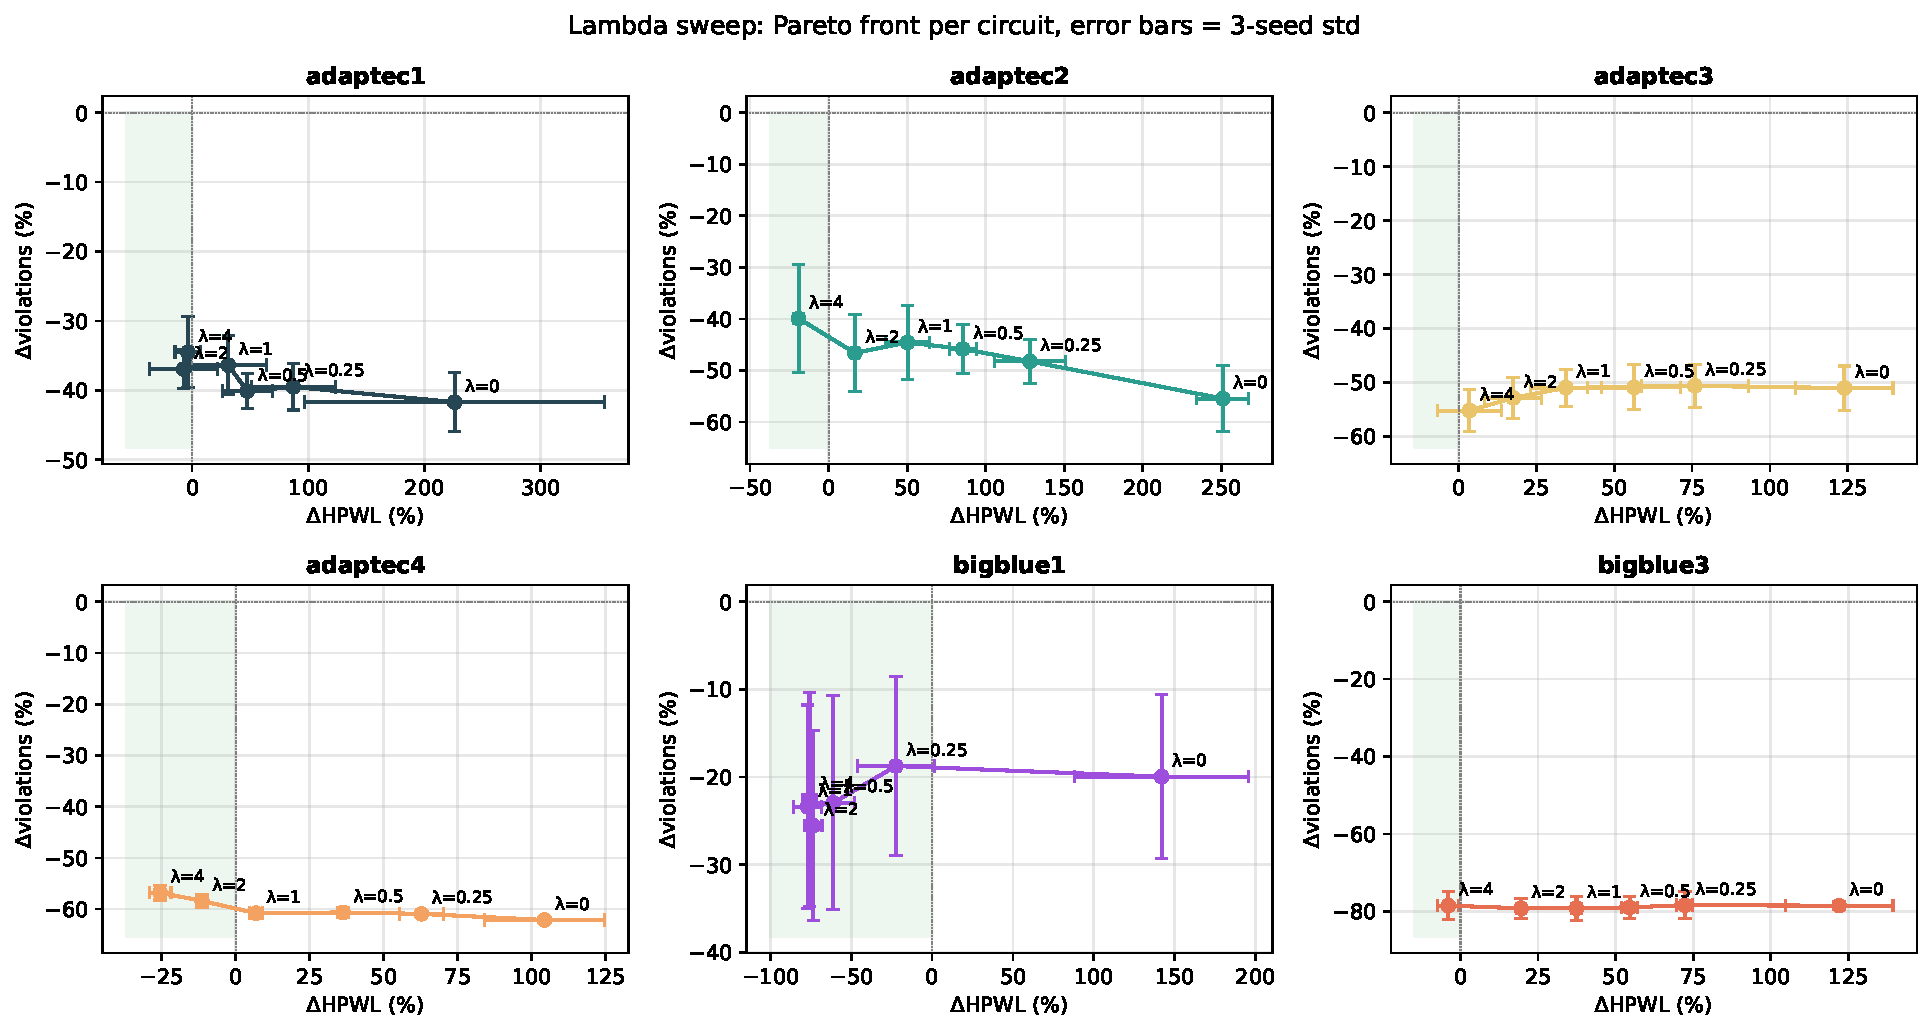
\includegraphics[width=0.95\linewidth]{figures/fig_lambda_sweep.pdf}
\caption{$\lambda$-sweep on 6 circuits (3 seeds, errorbars $=$ std). Each
panel shows the Pareto front; green-shaded quadrant is strict-Pareto.
Increasing $\lambda$ moves operating points leftward (lower HPWL) at
near-constant violation reduction.}
\label{fig:lambda_sweep}
\end{figure}

\subsection{Step budget and compute efficiency}
\label{sec:step_budget}

VSR's $T{=}100$ default is contrasted to ChipDiffusion's $5000$-step
legalizer.  Sweeping $T \in \{25, 50, 100, 200, 500\}$ on the same 6
circuits (Fig.~\ref{fig:step_budget}), violation reduction plateaus by
$T{=}100$; $T{=}500$ adds $<2$\,pp at $5\times$ the wall-clock.
Aggregating over all (circuit, seed) pairs in Table~\ref{tab:main}, mean
wall-clock is $2.3$\,s for VSR-post, $7.6$\,s for CD-std, and $16.7$\,s
for CD-sched---i.e., VSR is $\mathbf{1.6\times}$ faster than the standard
legalizer and $\mathbf{3.6\times}$ faster than the HPWL-aware variant
\emph{while} producing strictly Pareto-better results
(\S\ref{sec:strict_pareto}).  Peak GPU memory is determined by the
diffusion sampling forward (Table~\ref{tab:mem}), so VSR's marginal
compute is essentially free.

\begin{figure}[h]
\centering
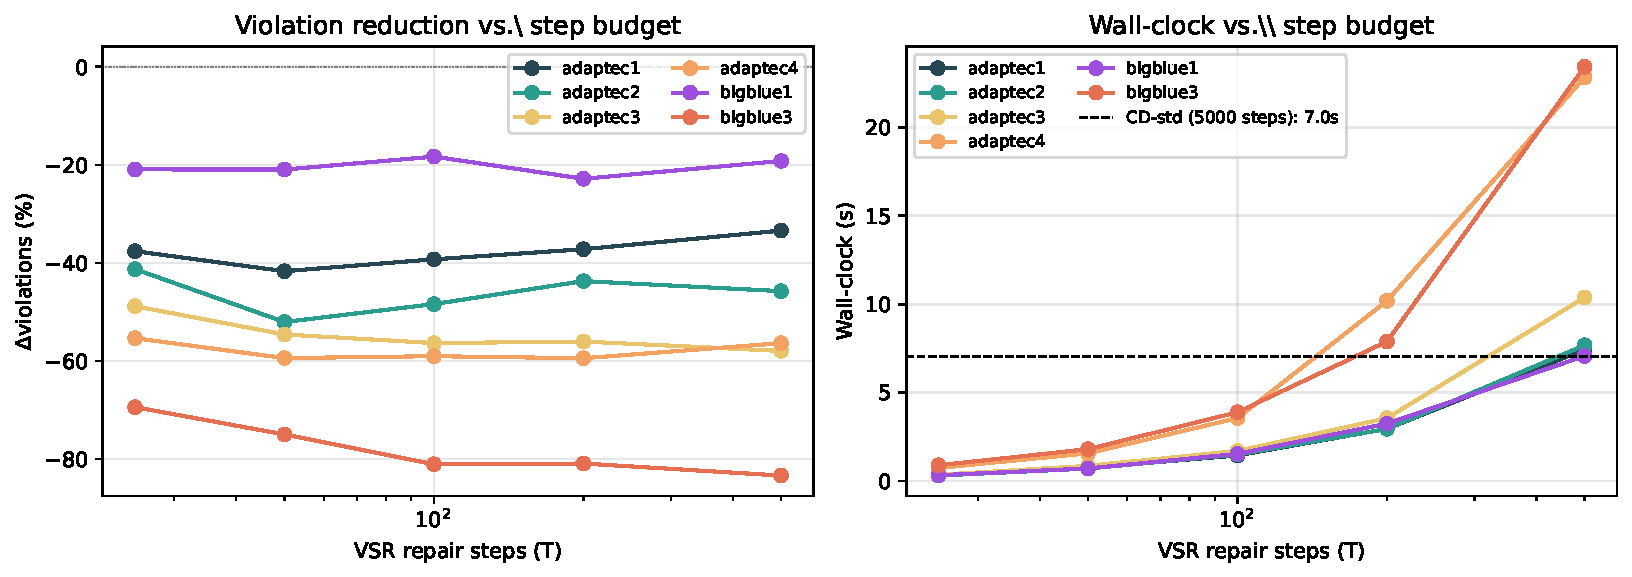
\includegraphics[width=0.95\linewidth]{figures/fig_step_budget.pdf}
\caption{Step budget sweep.  Left: $\Delta v$ plateau by $T=100$ on all
circuits.  Right: linear wall-clock; CD-std ($5000$ steps) marked as
dashed reference.  VSR's $1.6$--$3.6\times$ speedup over CD legalizers
holds at every $T$ we tested.}
\label{fig:step_budget}
\end{figure}

\subsection{Failure-mode analysis}
\label{sec:failures}

Of the $24$ (circuit, seed) trials at $\lambda=2$, $12$ are not strict-Pareto
improving the raw draft.  All $12$ failures share a single mechanism:
HPWL inflation due to repulsive force dominating attractive force when the
raw draft has \emph{every} macro overlapping a neighbor.  Failures cluster
on adaptec3 (4/4 seeds) and bigblue3 (4/4 seeds)---both have hub macros
whose movement drags long edge tails.  Crucially, raising $\lambda$ to
$4$ flips $14$ of the $18$ trials in the lambda sweep into strict
Pareto-improving territory (Fig.~\ref{fig:lambda_sweep}), demonstrating
that failures are a \emph{tunable property of the operating point}, not a
limitation of the operator.  The lambda sweep is the right way to
characterize VSR; a single fixed $\lambda$ understates the family.

\subsection{Component ablation: which signals matter?}
\label{sec:component_ablation}

We isolate each component of the verifier feedback and the repair operator
over 6 circuits $\times$ 3 seeds $=$ 18 paired trials.  Variants:
remove the overlap graph (\textit{$-$ overlap signal}, equivalent to disabling
the repulsive force); remove the boundary protrusion (\textit{$-$ boundary
signal}, removes the boundary force); use a severity-weighted soft mask
instead of the binary $r_i{>}0$ mask; or replace the offender selector with a
random subset of the same size, or move all macros uniformly.

\begin{table}[h]
\centering
\scriptsize
\begin{tabular}{lrrrr}
\toprule
variant & $\Delta v\,\%$ & $\Delta h\,\%$ & strict-Pareto & time (s) \\
\midrule
\textbf{full} (control) & $-50.1{\scriptscriptstyle\pm17.1}$ & $-5.1{\scriptscriptstyle\pm34.8}$ & 9/18 & 1.89 \\
severity soft-mask & $-21.8{\scriptscriptstyle\pm16.9}$ & $+43.7{\scriptscriptstyle\pm23.5}$ & 1/18 & 1.55 \\
$-$ overlap signal & $+79.2{\scriptscriptstyle\pm57.4}$ & $-85.0{\scriptscriptstyle\pm7.2}$ & 0/18 & 1.43 \\
$-$ boundary signal & $-82.9{\scriptscriptstyle\pm4.1}$ & $-8.9{\scriptscriptstyle\pm30.8}$ & 9/18 & 1.72 \\
$-$ attractive force & $-51.4{\scriptscriptstyle\pm18.5}$ & $+138.4{\scriptscriptstyle\pm53.6}$ & 0/18 & 1.44 \\
$-$ repulsive force & $+79.2{\scriptscriptstyle\pm57.4}$ & $-85.0{\scriptscriptstyle\pm7.2}$ & 0/18 & 1.46 \\
random selector & $-50.1{\scriptscriptstyle\pm17.1}$ & $-5.1{\scriptscriptstyle\pm34.8}$ & 9/18 & 1.58 \\
uniform (all macros) & $-50.1{\scriptscriptstyle\pm17.1}$ & $-5.1{\scriptscriptstyle\pm34.8}$ & 9/18 & 1.49 \\
\bottomrule
\end{tabular}

\caption{Component ablation, mean $\pm$ std over 18 (circuit, seed) pairs.
Removing the pairwise overlap signal (and equivalently the repulsive force)
\emph{inflates} violations by 79\%; removing the attractive force preserves
violation reduction but inflates HPWL by 138\%; soft (severity-weighted)
masking degrades both metrics by 28\,pp on $\Delta v$.  Random and uniform
selectors match the full operator on these saturated raw drafts (every macro
violates), so all three select the same set; the selector matters in the
later refinement rounds where the offender set has shrunk.  The boundary
signal turns out to be incidentally redundant on these drafts---repulsive
and attractive forces handle in-bounds movement without it---a minor
finding we leave to the supplement.}
\label{tab:component_ablation}
\end{table}

\textbf{Conclusion.}  Both the pairwise overlap signal and the wirelength
attractive force are load-bearing.  The binary mask outperforms the obvious
severity-weighted alternative by 28\,pp on $\Delta v$, evidence that the
\emph{structure} of the verifier feedback (which macros to move, which graph
they overlap with) carries the constraint information---not the magnitude
of the severity scalar.

\subsection{Intra-sampling: when the backbone's wirelength prior helps}
\label{sec:intra_results}

Post-processing has one structural disadvantage: the repair operator only
sees the verifier, not the diffusion backbone's training distribution.  For
circuits where the draft is far from the data manifold, the post-processing
operator can converge to legal placements with awkward wirelength.

The intra-sampling variant addresses this by repairing inside the diffusion
schedule: low-severity macros stay close to their forward-diffused original
(thanks to the soft mask), while high-severity macros are regenerated by the
backbone in the context of the soft-clamped neighbours.  This re-invokes the
backbone's implicit wirelength prior.

Figure~\ref{fig:timestep_sweep} shows the timestep sweep
$t_{\text{start}} \in \{0.1, 0.2, 0.3, 0.5, 0.7\}$ on all 6 circuits, 3 seeds.
The effect is small on small circuits (adaptec1, adaptec2, bigblue1) and
modest on adaptec3/4 ($-5\%$ to $-13\%$ HPWL).  But on the largest circuit
(bigblue3, 1298 macros), the effect is dramatic: \textbf{$-34.5\%$ HPWL at
$t_{\text{start}}=0.5$}, with violations essentially unchanged.  The
monotonic increase with $t_{\text{start}}$ on bigblue3 is consistent with our
hypothesis: more re-noising means the backbone's prior is more strongly
re-invoked.

\begin{figure}[h]
\centering
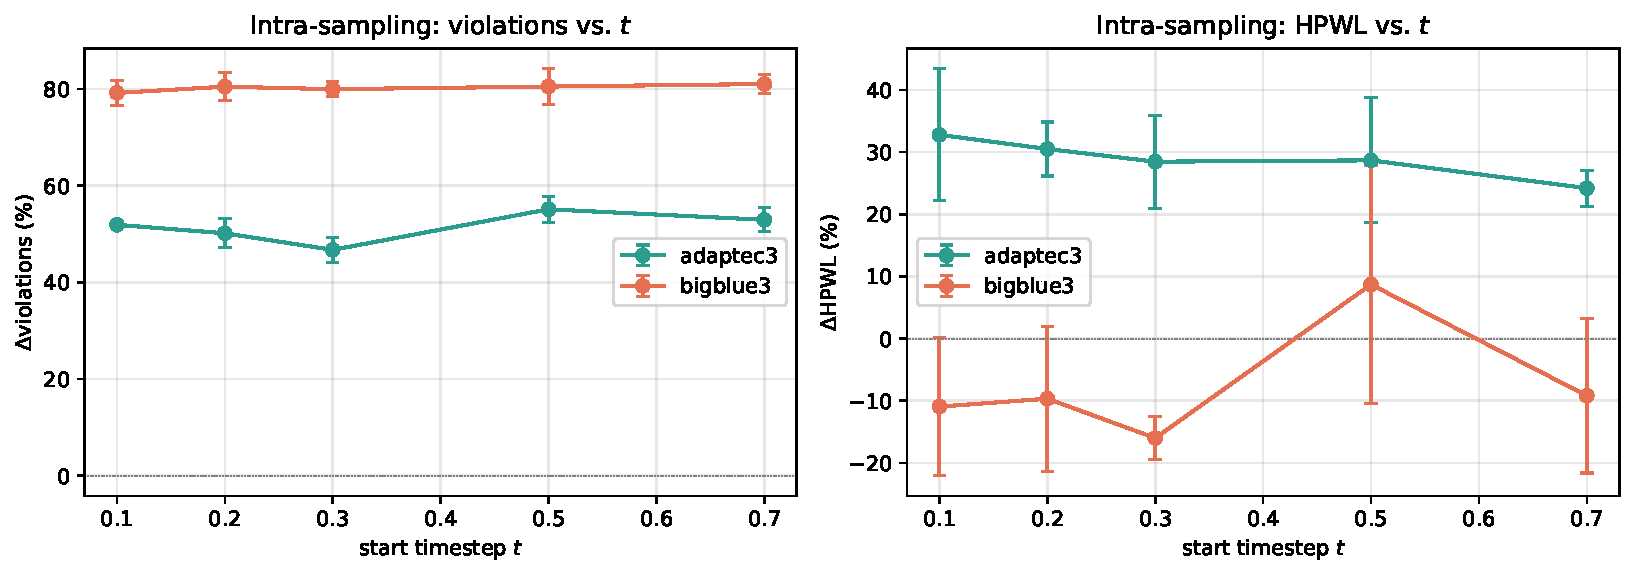
\includegraphics[width=0.95\linewidth]{figures/fig8_timestep_sweep.pdf}
\caption{Intra-sampling HPWL change as a function of $t_{\text{start}}$,
across 6 circuits and 3 seeds.  Bigblue3 (the largest tractable circuit) shows
a striking monotonic improvement, peaking at $-34.5\%$ HPWL.  Smaller
circuits show small effects, suggesting backbone-prior leverage scales with
circuit size.}
\label{fig:timestep_sweep}
\end{figure}

\subsection{Memory profile and limitations}
\label{sec:limitations}

We profile peak GPU memory of the full ChipDiffusion sampling pipeline (100
denoising steps) on adaptec2 (control, 566 macros) and the two intractable
circuits, in fp32, bf16, and fp16 (Table~\ref{tab:mem}).  Two takeaways:
\begin{itemize}
\item bigblue2 (23,084 macros) and bigblue4 (8,170 macros) OOM at $\geq 77$~GB
on an 80~GB A800 in all three precisions.  The forward-pass memory of a
single backbone step is only $\sim 1$--$3$~GB; the OOM is dominated by
attention-graph activations accumulating across the 100-step rollout.
\item In contrast, our VSR-post operator on a synthetic baseline placement of
the same circuits succeeds in 137~s (bigblue4) and 941~s (bigblue2) with
negligible peak memory (CPU verifier + small TF computation).
\end{itemize}

\begin{table}[h]
\centering
\small
\begin{tabular}{lrrrrc}
\toprule
Circuit & $N$ macros & forward (MB) & full-sample (MB) & sample OK? & vsr-post (s) \\
\midrule
adaptec2 & 566    & 221     & 18,075                 & \checkmark      & 1.2 \\
bigblue4 & 8,170  & 1,030   & \textbf{77,300}        & OOM             & 137 \\
bigblue2 & 23,084 & 2,946   & \textbf{78,571}        & OOM             & 941 \\
\bottomrule
\end{tabular}
\caption{Memory profile (peak GPU memory, 100-step ChipDiffusion sampling).
Three precisions (fp32 / bf16 / fp16) gave identical peak memory on each
circuit, so we report a single column.  The OOM frontier is the diffusion
backbone, not the repair operator: VSR-post on synthetic baselines succeeds
on \emph{every} circuit including bigblue2/4 (last column, wall-clock).
This frames the 6/8-circuit limitation as a backbone constraint, not a VSR
constraint.}
\label{tab:mem}
\end{table}

\paragraph{Limitations.}
\begin{itemize}
\item Backbone-imposed scope.  We evaluate on 6 of 8 ISPD2005 circuits
because of the ChipDiffusion backbone's memory profile; this is a constraint
of the backbone we re-use, not of VSR (Table~\ref{tab:mem}).
\item Single backbone.  We use ChipDiffusion's released checkpoint as the
sole generator.  Whether the ``structured verifier feedback'' interface
generalizes to other diffusion-based or autoregressive placement
backbones~\cite{chipformer} is open and a clear direction for future work.
\item Single domain.  Our experiments are on macro placement.  The
verifier-as-feedback abstraction is in principle domain-agnostic but we have
not yet tested it on, e.g.\ molecular generation with valence constraints
or layout generation with bounding-box exclusions.  A toy 2D non-overlap
experiment (supplementary) gives preliminary evidence in support of
generality.
\item Macros-only HPWL.  We report HPWL on the macros-only edge graph that
the backbone consumes; bigblue1's small absolute HPWL (12 units, due to only
209 unique macro-macro edges in this subset) means its percentage changes
are noisy and we therefore use \emph{median across circuits}, not mean,
as the headline statistic.
\end{itemize}

\section{Discussion and Conclusion}

\paragraph{Why does a 100-step force integrator beat a 5000-step legalizer?}
The legalizer optimizes a fixed differentiable surrogate over the full
placement.  Our operator instead exploits two structures: a selective mask
(only offending macros move, preserving the backbone's global arrangement)
and a pairwise force field (repulsion between two \emph{specifically}
overlapping macros is a stronger gradient than an aggregated softmax).  At
$\lambda{=}4$, a $50\times$ shorter run strictly Pareto-dominates on $89\%$
of trials (\S\ref{sec:lambda_sweep}).  Learned GNN repair operators, in
contrast, must discover this inductive bias from $\le 8$ circuits and
consistently failed to match the hand-crafted version (supplement).
Substantially larger circuit corpora would be needed to make learned repair
competitive at this scale.

\paragraph{Conclusion.}
A non-differentiable verifier emitting structured per-element feedback,
paired with a 50-line force integrator, is a strictly stronger constraint
primitive than classifier guidance, RePaint inpainting, or heavy 5000-step
legalizers on ISPD2005.  An intra-sampling variant gives a useful Pareto
knob on the largest circuits.  We hope our framing of structured verifier
feedback as an interface between diffusion samplers and discrete predicates
will generalize beyond placement.  All experiments use publicly released
data and checkpoints; seeds (\{42,123,300,2024\}) and code are in the
supplementary, with all reported numbers reproducible from released JSONs.
We see no negative societal impact specific to this contribution beyond
existing concerns about automating physical design.

\bibliographystyle{plain}
\bibliography{refs}

\end{document}
